\chapter{\label{chap:chap3} Proposta de trabalho}

Seguindo a organização arquitetural da Figura \ref{fig:fig1}, a proposta deste trabalho é fazer com que um \textit{fog node} conheça, de forma autônoma, os recursos disponibilizados por seus vizinhos.
Assim, cada \textit{fog node} saberá quais são os \textit{edge devices} disponíveis na rede, portanto,
o nodo que possui o sensor de chuva saberia que existe um outro nodo na rede capaz de medir a temperatura, por exemplo.


Podemos observar na topologia da Figura \ref{fig:fig1}, que os \textit{fog nodes} não possuem uma um nodo central como servidor.
Em razão da topologia distribuída, se for necessário escalarmos a quantidade de nodos na rede, a mesma não deverá sofrer impactos significativos de performance.

Nas seções a seguir abordaremos a arquitetura, módulos e submódulos que compõem o projeto, bem como resultados esperados, validações e cenários de teste. 

\section{Arquitetura}

Esta Seção define a pilha de protocolos a serem utilizados neste projeto, bem como a justifica pela escolha dos mesmos.
A pilha de protocolos atuará em conjunto com a organização arquitetural previamente definida na Figura \ref{fig:fig1}.

A fim de facilitar a compreensão da arquitetura deste projeto, a Figura \ref{fig:fig2} explicita a pilha de protocolos que o projeto fará uso para implementar as funcionalidades propostas.

\begin{figure}[htb!]
    \centering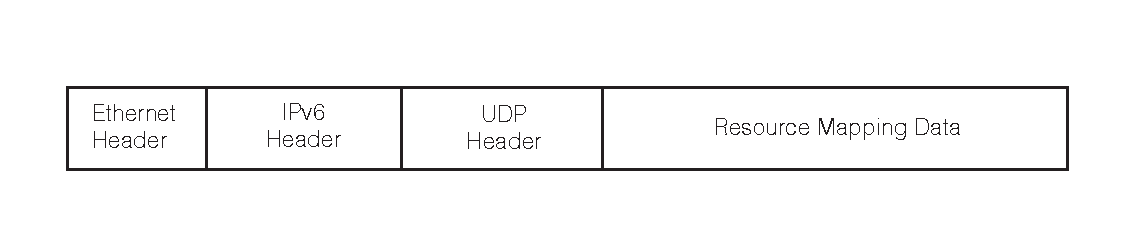
\includegraphics[width=.8\textwidth]{fig2.png}
    \caption%[This figure has a shorter caption now]%
    {\label{fig:fig2} Pilha de protocolos.}
\end{figure}

O modelo de referência TCP/IP é constituido de cinco camadas: física, enlace, rede, transporte e aplicação \cite{tanenbaum2011redes}.
Nesse trabalho, o níveis de rede e transporte (IPv4 e UDP respectivamente) serão utilizados para a implementação do modelo proposto.

A utilização de IPv4 na camada de rede justifica-se pelo fato do protocolo ser empregado em redes locais, que geralmente não necessitam de uma quantidade de endereçamento tão grande 
se comparado ao IPv6, mas não existem impedimentos para que implementações futuras utilizem IPv6 na camada de rede.

Manter o contexto de conexão entre os nodos, utilizando TCP por exemplo, despenderia uma quantidade de trafego desnecessário na rede.
Visto que a simplicidade é um dos objetivos deste trabalho e que transitar uma pequena quantidade de dados a cada requisição aumenta o desempenho da solução,
a utilização de datagramas UDP faz sentido neste protocolo

O protocolo proposto, entitulado \textit{Resource Mapping}, como apresentado na Figura \ref{fig:fig2}, atuará na camada de aplicação do modelo de referência TCP/IP \cite{tanenbaum2011redes} e será responsável por padronizar, descobrir e sincronizar os nodos da névoa.
Os maiores desafios neste modelo proposto são manter o estado global dos recursos acessível a todos os nodos, e garantir que o desempenho seja satisfatório com o objetivo permitir a escalabilidade da solução.



\section{Módulos}

De forma geral, cada nodo da rede deverá manter uma lista com os endereços IP`s que fazem parte do mapeamento.
Atrelado à cada endereço IP, deverá haver uma lista com os recursos providos por este.
Em vista disso, cada nodo portará um mapeamento global de recursos disponíveis na névoa.

O detalhamento das funcionalides que o projeto deverá dispor, bem como ilustrações relacionadas aos fluxos, serão abordadas nas proximas subseções.

\subsection{Middleware}

Observando a Figura \ref{fig:fig1}, notamos que há comunicação entre um fog node e seus respectivos edge devices.
A comunicação entre estes não é o foco deste projeto, portanto, será tratada de forma simulada.
Assim sendo, a simulação deverá prever alguns casos que, por vezes, possam suceder. Dentre alguns dos eventos possíveis está
o acréscimo ou remoção de um edge device vinculado à algum fog node.

A manutenção dos recursos, acréscimo ou remoção, transcorrerá utilizando o protocolo CoAP.
Utilizar CoAP para estas funcionalidades faz sentido, uma vez que este prevê meios para vinculação de recursos a nodos.

Segundo a definição de POST do protocolo CoAP, sua função é determinada pelo servidor que está recebendo a requisição e pelo do recurso referenciado na URI.
Geralmente a sua utilização resulta na criação ou atualização de um recurso.\cite{rfc7252}.
Já a mesma RFC define o método DELETE como sendo um método de remoção de recursos baseado em URIs\cite{rfc7252}.
Nessa perspectiva, portanto, o uso do método POST faz sentido para gerarmos \textit{(CoRE) Link Format} e o método DELETE para removermos.


\subsection{Descoberta de recursos}


Partindo do pressuposto que os nodos da névoa já possuem seus recursos devidamente criados e acessíveis via CoAP,
como primeiro passo do mapeamento devemos considerar a entrada de um novo nodo na rede.
No momento em que o nodo dispor de um endereço IP válido, este deverá enviar um pacote para o endereço de broadcast indicando que possui recursos a serem disponibilizados.


Ao receberem o pacote enviado por broadcast, os nodos que desejarem saber quais recursos estão sendo providos por este novo membro, deverão realizar uma Requisição
unicast para a URI \textit{/.well-known/core} utilizando o protocolo CoAP.
Vale lembrar que este fluxo de requisição e resposta, utilizando a URI \textit{/.well-known/core}, faz com que o nodo requisitado retorne todos seus recursos ao solicitante.


Com o objetivo de exemplificar a primeira fase do protocolo, as Figuras \ref{fig:fig5} e \ref{fig:fig6} apresentam o fluxo para a descoberta de recursos.

%  mencionar q cada fog tem edge devices
A topologia da névoa utilizada nas imagens é definida por fog nodes enumerados de um à cinco, sendo o nodo FN5 o ultimo a entrar na rede.
A figura \ref{fig:fig5} demonstra o nodo FN5 entrando na névoa e, portanto, deverá anunciar-se por broadcast indicando que possui recursos a serem disponibilizados.

\begin{figure}[htb!]
    \centering\includegraphics[width=.5\textwidth]{fig5.png}
    \caption%[This figure has a shorter caption now]%
    {\label{fig:fig5} Nodo entrando na névoa.}
\end{figure}

Após FN5 enviar mensagem Olá por broadcast, os nodos FN1, FN2 e FN4 realizam a Requisição diretamente ao FN5 afim de obter os recursos disponíbilizados por ele,
já o nodo FN3, por não estar executando o protocolo de mapeamento, não.


\begin{figure}[htb!]
    \centering\includegraphics[width=.5\textwidth]{fig6.png}
    \caption%[This figure has a shorter caption now]%
    {\label{fig:fig6} Nodos realizando Requisição.}
\end{figure}


\subsection{Gerenciamento de recursos}

A manutenibilidade da lista de recursos globais é relevante para que a implementação do protocolo tenha sucesso, pois, a névoa deverá saber quando um nodo, ou recurso dele, deixou de fazer parte rede.
Para tal, faz-se necessário a utilização de alguns mecanismos de controle.
Esses controles são realizados em duas esferas, a primeira trata da inserção ou remoção de um nodo na rede,
já a segunda refere-se a inserção ou remoção de um edge device, vinculado a um nodo qualquer.
% SJF: Ta um pouco confuso esse parágrafo. Tenta remover as vírgulas, reescrevendo e mudando um pouco o estilo.



Inicialmente abordaremos a entrada e saída de nodos da névoa, e para esta subseção será utilizado o cenário da Figura \ref{fig:fig6} quando necessário.
O Pseudocódigo \ref{alg:alg1} demonstra, de forma sucinta, a política de atualização que cada nodo deverá implementar.

\begin{algorithm}[htb]
    \begin{center}
        \begin{algorithmic}[1]
            \STATE \textbf{function} $\text{Police(ip, resources)}$
            \STATE \hspace{\algorithmicindent} \textbf{if} $\text{exists(ip)}$
            \STATE \hspace{\algorithmicindent} \hspace{\algorithmicindent} $\text{update(ip, resources)};$
            \STATE \hspace{\algorithmicindent} \textbf{else}
            \STATE \hspace{\algorithmicindent} \hspace{\algorithmicindent} $\text{insert(ip, resources)};$
        \end{algorithmic}
    \end{center}
    \caption[Política de atualização de recursos]%
        {\label{alg:alg1} Política de atualização de recursos.}%
    \end{algorithm}

No momento em que o nodo recebe a resposta de sua Requisição, contendo os recursos providos pelo nodo requisitado, aquele deverá armazenar as informações em uma estrutura de dados adequada.
Essa estrutura de dados estará implementada em todos os nodos da névoa, e a partir dela será possível realizar o gerenciamento dos recursos de forma simples e eficiente.
O trecho abaixo define, por ora, o formato dos dados que serão utilizados em cada nodo.


% SJF: Requisição -> requisição


\begin{verbatim}
    Fog = {
        string ip;
        string resources[];    
    }
    Fog fogs[];
    string myResources[];
\end{verbatim}

De posse da Figura \ref{fig:fig6} como cenário, do algoritmo de atualização \ref{alg:alg1}, e da estrutura de dados previamente descrita,
demonstramos abaixo o estado em que se encontram os dados armazenados em FN2 após a aplicação do método.

\begin{verbatim}
    fogs: [
        {
            ip: '192.168.0.1',
            resources: [ 'ED1' ]
        },
        {
            ip: '192.168.0.3',
            resources: [ ]
        },
        {
            ip: '192.168.0.4',
            resources: [ 'ED1' ]
        },
        {
            ip: '192.168.0.5',
            resources: [ 'ED1', 'ED2' ]
        }
    ];
    myResources: [ 'ED1', 'ED2', 'ED3' ];
\end{verbatim}

Visto isso, é imprescindível que os nodos mantenham seus dados consistentes, pois, após adicionar o novo nodo em sua lista de fogs, o protocolo precisa ser capaz de perceber quando um elemento
deixou de fazer parte do processo. Assim, a manutenção dos estados será abordado de forma similar as mensagens de \textit{keep alive} utilizadas no protocolo BGP, por exemplo.
Mensagens de keep alive são adotadas para que os nodos da rede avisem seus vizinhos que ainda estão em operação, pois, sem esse procedimento seria difícil
saber quando remover um IP da lista de recursos. Portanto, para manter a lista atualizada, este protocolo implementará mensagens desse tipo.

As mensagens de keep alive serão transmitidas sob broadcast em um intervalo de trinta segundos, porém, este é apenas um valor inicial, e conforme o desenvolvimento do projeto esse
parâmetro pode ser ajustado para que a solução obtenha uma eficiência satisfatória.
Após o recebimento da mensagem de keep alive, os nodos deverão respondê-las indicando que ainda estão em operação.
Caso o nodo não responda a mensagem de keep alive, este será marcado como parcialmente inativo pelo remetente da mensagem.
Quando o nodo solicitante realizar outra mensagem de keep alive e o nodo que já estava marcado com parcialmente inativo não responder, o mesmo será removido da lista de recursos do
solicitante, e assim é possível saber quando um nodo deixou de fazer parte da névoa.
Para realizar este controle será preciso adicionar na estrutura \textit{Fog} a propriedade boleana, denominada \textit{isReplyingKeepAlive}, que indica se o nodo está respondendo a solicitações de keep alive.

As mensagens de keep alive mantém os nodos informados sobre o estado de seus vizinhos, mas não conseguem indicar informações relacionadas aos edge device.
Consequentemente, não é possível saber quando um edge device parou ou iniciou sua operação em um nodo ativo.

Para que seja possível detectarmos esse tipo de comportamento, o protocolo proposto deverá implementar a técnica denominada \textit{época},
e servirá para que os nodos mantenham ciênia sobre o estado dos edge devices de seus vizinhos de rede.
Para isso, uma nova propriedade denominada \textit{epoch}, do tipo inteiro, deverá ser adicionada a estrutura de dados, e estará presente tanto no nodo em sí quanto em cada item da lista de fogs.
O valor da época será incrementado em uma unidadade a toda alteração observada no nodo, seja pelo acréscimo ou pela remoção de edge devices.

A partir de agora, então, todas as mensagens de keep alive deverão conter a época do nodo que está realizando o broadcast.
Assim, todo nodo que receber a mensagem poderá comparar a época recebida na mensagem com a época que possui armazenada em sua lista de fogs referente ao remetente da mensagen.
Havendo divergencia de épocas, este poderá realizar uma nova requisição para atualizar sua lista de recursos referente aquele nodo em específico.

Após as alterações realizadas na estrutura de dados, abaixo temos o novo modelo que suportará as funcionalidades propostas.
\begin{verbatim}
    Fog = {
        string ip;
        string resources[];
        int epoch;
        boolean isReplyingKeepAlive;
    }
    Fog fogs[];
    string myResources[];
    int epoch;
\end{verbatim}

Além do protocolo de mapeamento em sí, este trabalho disponibilizará uma API para o gerenciamento de recursos locais.
Esta API deverá ser executada localmente e possuirá métodos para listagem, remoção e criação de recursos, portanto, a partir dela será possível
simularmos o gerenciamento, inserção e remoção, de recursos que o protocolo implementará.

\section{Resultados esperados}

Espera-se que este trabalho resulte em um protocolo funcional, simples e que seja capaz de descobrir e sincronizar recursos de dispositivos sob computação em névoa.
Além disso, temos como objetivo fazer com que a névoa configure-se de forma autônoma, ou seja, quando um recurso ou nodo entrar ou sair da rede, a mesma deverá manter-se coerente.
Esta coerência significa manter o estado global dos recursos acessível a todos os nodos.

A névoa será construída de forma simulada utilizando a ferramenta Common Open Research Emulator (CORE)\cite{coregui}. Nela é possível criar as mais variadas topologias de redes,
além disso, cada nodo adicionado à topologia contém um terminal Unix que pode ser utilizado para executar comandos. Então, os comandos da API descritos acima,
podem ser utilizados a fim de auxiliar o gerenciamento dos recursos locais dos nodos. A ferramenta de monitoramento de trafego de rede, Wireshark\cite{wireshark}, será utilizada em conjuntos com o 
CORE, pois, nela será possível apurarmos se os pacotes estão sendo enviados e recebidos da forma correta.


\section{Validação}

A validação deste trabalho consiste em realizar simulações que faça com que o protocolo execute suas funcionalidades de acordo com os resultados descritos na Seção anterior, sendo assim, 
algumas situações devem ocorrer para que as validações sejam realizadas.
Estas situações serão abordadas nos cenários de teste da Seção a seguir.

\section{Cenários de teste}

Utilizando como base a Figura \ref{fig:fig7}, e partindo do pressuposto que todos os nodos da névoa já estão com seus recursos sincronizados corretamente,
iremos exemplificar os cenários de testes elencados abaixo.

\begin{enumerate}
    \item Entrada de algum equipamento na rede e este anunciando seus recursos. 
    \item Atualização das listas globais quando algum equipamento deixar de responder as mensagens de keep alive.
    \item Atualização da lista de recursos quando algum edge device é adicionado ou removido de um nodo da névoa.
\end{enumerate}

\begin{figure}[htb!]
    \centering\includegraphics[width=.8\textwidth]{fig7.png}
    \caption%[This figure has a shorter caption now]%
    {\label{fig:fig7} Topologia base para cenário de teste.}
\end{figure}

O Item 1 não será demonstrado agora, uma vez que as Subseções 3.2.2 e 3.2.3 já o fizeram, portanto, partiremos diretamente para o segundo item da listagem.

O segundo item trata de quando um nodo deixa de responder mensagens de keep alive, e a Figura \ref{fig:fig7} será utilizada para ilustrar este funcionamento.
Na Figura \ref{fig:fig8}, o nodo FN1 não respondeu, no tempo previamente estipulado, a mensagem de keep alive enviada pelo nodo FN2, 
portanto, o nodo destinatário foi marcado em FN2 como parcialmente inativo.
\begin{figure}[htb!]
    \centering\includegraphics[width=.8\textwidth]{fig8.png}
    \caption%[This figure has a shorter caption now]%
    {\label{fig:fig8} Nodo deixa de responder mensagens de keep alive.}
\end{figure}
Já a figura \ref{fig:fig9} demonstra que o nodo FN1 não respondeu novamente à mensagem de keep alive enviada por FN2, por isso, foi removido de sua lista de recursos. 
\begin{figure}[htb!]
    \centering\includegraphics[width=.8\textwidth]{fig9.png}
    \caption%[This figure has a shorter caption now]%
    {\label{fig:fig9} Nodo removido da lista de recursos.}
\end{figure}
O terceiro item dos cenários de teste trata de quando o nodo está normalmente em operação, porém, um de seus recursos foi alterado, seja por incremendo de um novo edge device ou
pela remoção de um.

Utilizaremos a Figura \ref{fig:fig5} como exemplo básico, e nela podemos observar que o edge device denominada ED3 vinculado ao nodo FN2 parou de funcionar.
Para este cenário, o nodo que hospeda ED3 deve estar ciente que este edge device está inoperante, e assim atualizar a sua \textit{época}.
O nodo que possui o edge device inoperante, então, terá sua época enviada juntamente das mensagens de keep alive.
Assim, quando os nodos receberem o keep alive poderão compará-los e posteriormente realizar requisição ao nodo para atualizar sua lista de recursos globais.

\begin{figure}[htb!]
    \centering\includegraphics[width=.8\textwidth]{fig10.png} 
    \caption%[This figure has a shorter caption now]%
    {\label{fig:fig10} Atualização de recursos após edge device ser removido da névoa.}
\end{figure}



